\paragraph{Example 1: Polynomial Fit of Varying degree}{
\begin{lstlisting}[language=Python]
from BNumMet.Visualizers.LeastSquaresVisualizer import LSPVisualizer
xData = np.array([0, 1, 2, 3, 4, 5])
yData = np.array([4.5, 2.4, 1.5, 1, 1.5, 2.4])
lspVisualizer = LSPVisualizer(xData, yData)
lspVisualizer.run()
\end{lstlisting}

\begin{enumerate}
    \item Initial State\\
    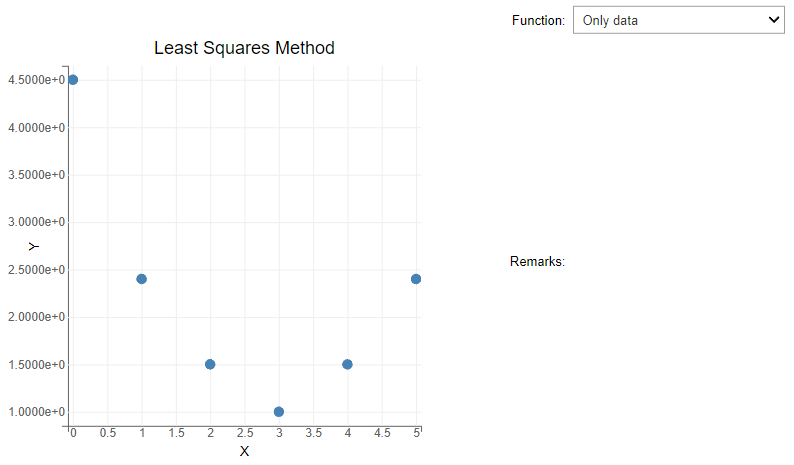
\includegraphics[scale=0.6]{Include/Images/Thesis/Documentation/Visualizers/LeastSquares/Example 1/Example 1 - 00 - Initial State.png}
    \item Selector\\
    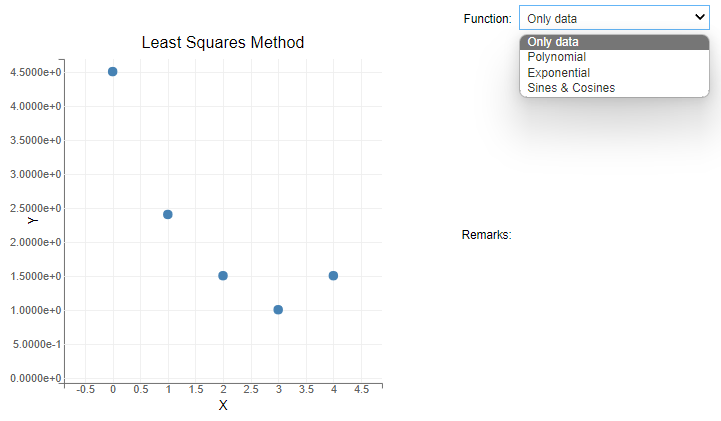
\includegraphics[scale=0.6]{Include/Images/Thesis/Documentation/Visualizers/LeastSquares/Example 1/Example 1 - 00 - Selector.png}
    \item Select Polynomial\\
    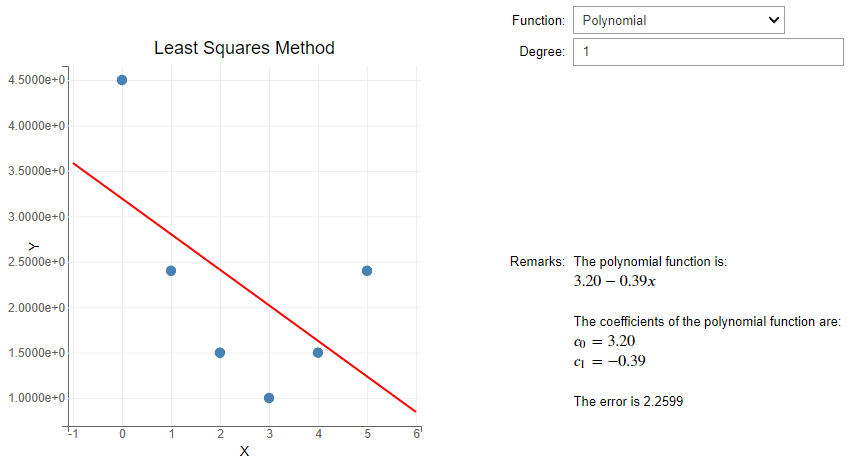
\includegraphics[scale=0.6]{Include/Images/Thesis/Documentation/Visualizers/LeastSquares/Example 1/Example 1 - 00 - Polinomial .png}
    \item Increment degree by 1 (degree 2)\\
    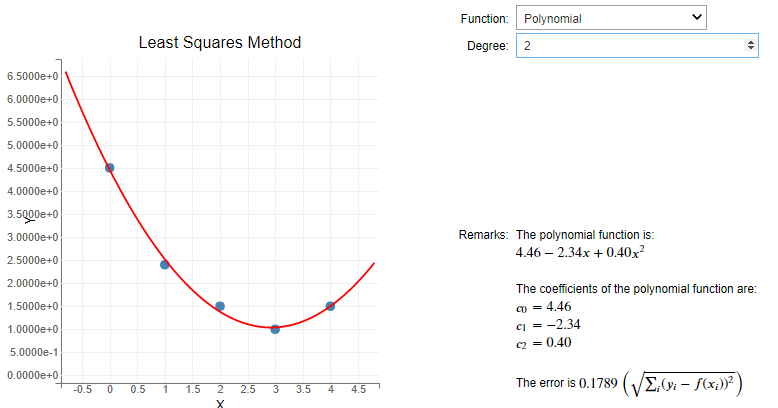
\includegraphics[scale=0.6]{Include/Images/Thesis/Documentation/Visualizers/LeastSquares/Example 1/Example 1 - 01 - Polinomial Degree 2.png}
    \item Degree 5 (Maximum, cannnot go higher)\\
    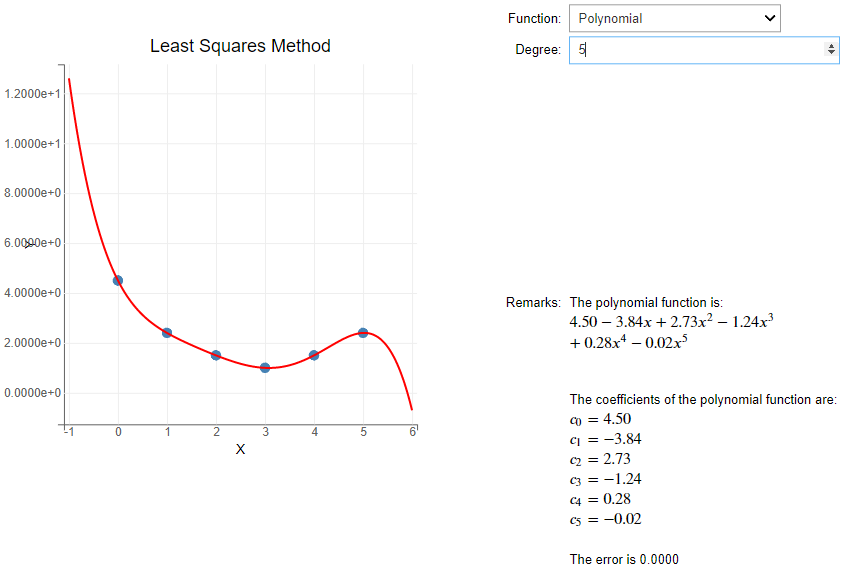
\includegraphics[scale=0.6]{Include/Images/Thesis/Documentation/Visualizers/LeastSquares/Example 1/Example 1 - 02 - Polinomial Degree 5.png}

\end{enumerate}
}

\paragraph{Example 2: No Input Data and Exponential Fit}
\begin{lstlisting}[language=Python]
from BNumMet.Visualizers.LeastSquaresVisualizer import LSPVisualizer
lspVisualizer = LSPVisualizer()
lspVisualizer.run()
\end{lstlisting}
\begin{enumerate}
    \item Initial state\\
    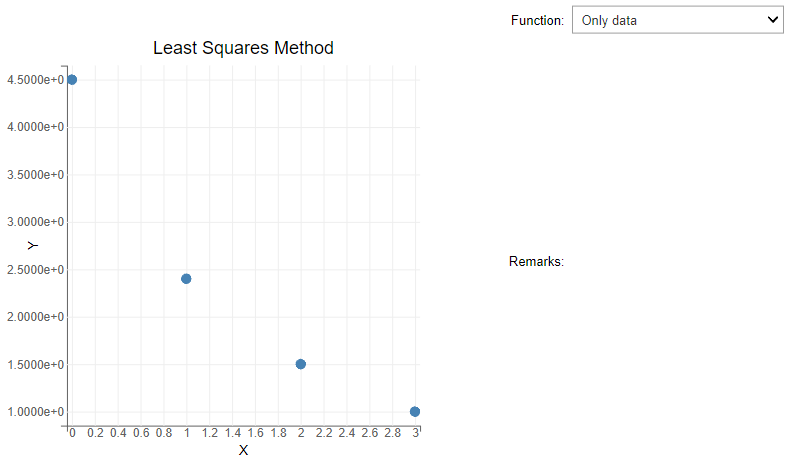
\includegraphics[scale=0.6]{Include/Images/Thesis/Documentation/Visualizers/LeastSquares/Example 2/Example 2 - 00 - Initial State.png}
    \item Exponential Selection\\
    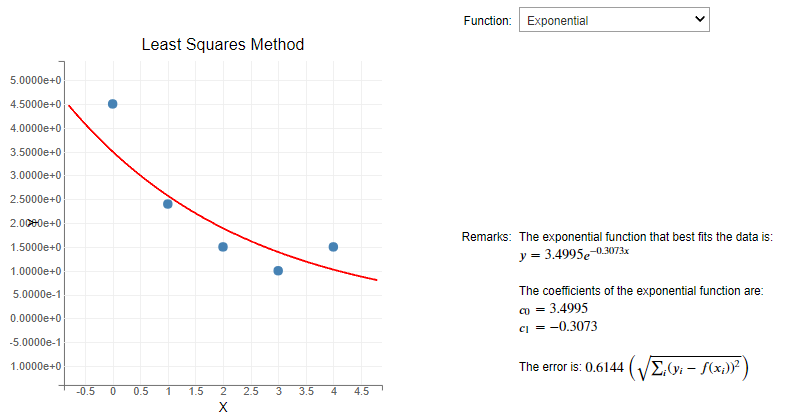
\includegraphics[scale=0.6]{Include/Images/Thesis/Documentation/Visualizers/LeastSquares/Example 2/Example 2 - 00 - Exponential.png}
\end{enumerate}

\paragraph{Example 3: Sines and Cosines Fit of Varying degree}{
\begin{lstlisting}[language=Python]
from BNumMet.Visualizers.LeastSquaresVisualizer import LSPVisualizer
xData = np.array([0, 1, 2, 3, 4, 5])
yData = np.array([4.5, 2.4, 1.5, 1, 1.5, 2.4])
lspVisualizer = LSPVisualizer(xData, yData)
lspVisualizer.run()
\end{lstlisting}

\begin{enumerate}
    \item Initial State\\
    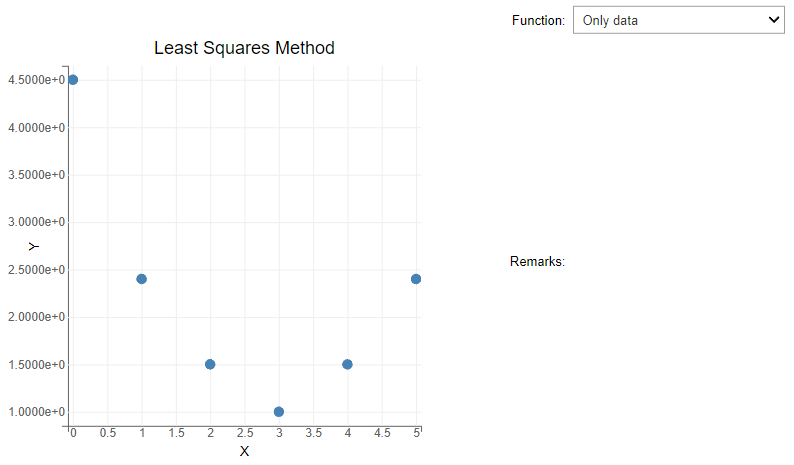
\includegraphics[scale=0.6]{Include/Images/Thesis/Documentation/Visualizers/LeastSquares/Example 1/Example 1 - 00 - Initial State.png}
    \item Selector\\
    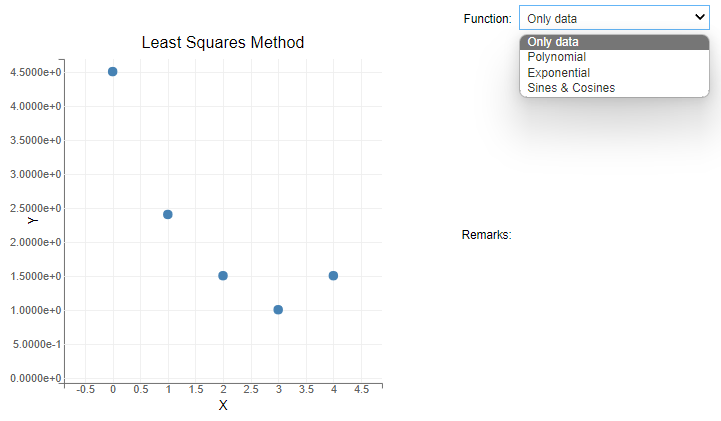
\includegraphics[scale=0.6]{Include/Images/Thesis/Documentation/Visualizers/LeastSquares/Example 1/Example 1 - 00 - Selector.png}
    \item Select Sines \& Cosines\\
    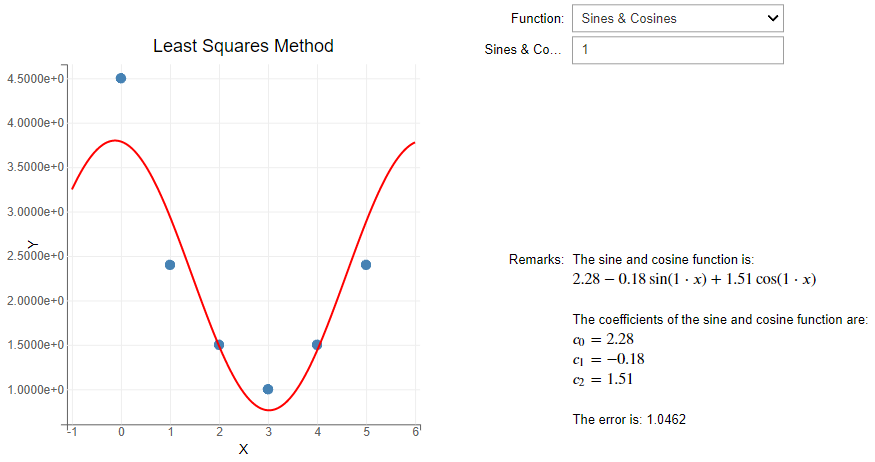
\includegraphics[scale=0.6]{Include/Images/Thesis/Documentation/Visualizers/LeastSquares/Example 3/Example 3 - 00 - Trigonometry.png}
    \item Set degree to the maximum\\
    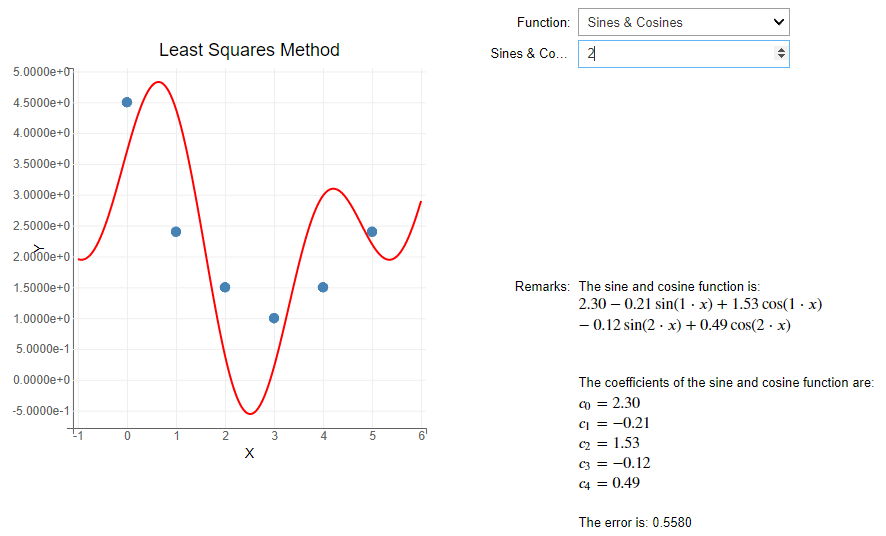
\includegraphics[scale=0.6]{Include/Images/Thesis/Documentation/Visualizers/LeastSquares/Example 3/Example 3 - 01 - Trigonometry Degree 2.png}
\end{enumerate}
}
